\subsubsection{UCA 5 - Monitoraggio dello storico degli accessi dell'utente}

\begin{figure}[h]
	\centering	
	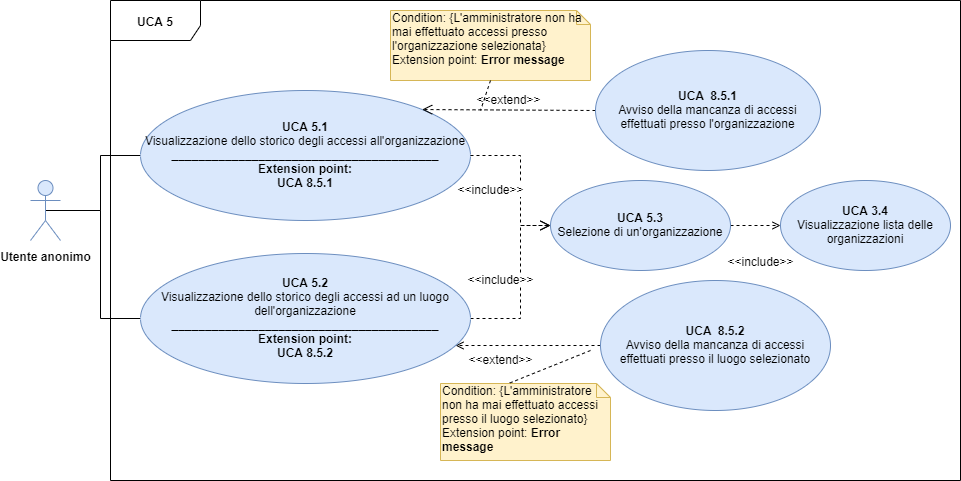
\includegraphics[scale=0.4, center]{sezioni/UseCase/Immagini/UCA5.png}
	\caption{UCA 5 - Monitoraggio dello storico degli accessi\ap{G} dell'utente}
\end{figure}

\begin{itemize}
    \item \textbf{Attori primari:} Utente anonimo
    \item \textbf{Precondizione:} L'utente ha precedentemente scaricato la lista delle organizzazioni\ap{G}.
    \item \textbf{Postcondizione:} L'utente ha visualizzato lo storico degli accessi\ap{G} relativo all'organizzazione\ap{G} desiderata oppure al luogo\ap{G} desiderato dell'organizzazione\ap{G} scelta.
    \item \textbf{Scenario principale:} L'utente selezionerà l'organizzazione\ap{G} desiderata dalla lista delle organizzazioni\ap{G} e quindi la funzionalità per mostrare lo storico degli accessi\ap{G} oppure un luogo\ap{G} specifico per analizzarne il relativo storico degli accessi\ap{G}.
\end{itemize}

\subsubsection{UCA 5.1 - Visualizzazione dello storico degli accessi all'organizzazione}
\begin{itemize}
    \item \textbf{Attori primari:} Utente anonimo
    \item \textbf{Precondizione:} L'utente ha precedentemente scaricato la lista delle organizzazioni\ap{G}.
    \item \textbf{Postcondizione:} L'utente ha visualizzato lo storico degli accessi\ap{G} (con nome dell'organizzazione\ap{G}, timestamp\ap{G} di ingresso, di uscita, e tempo di permanenza) presso l'organizzazione\ap{G} scelta. Se si trova all'interno dell'organizzazione\ap{G} stessa, viene visualizzato il tempo passato al suo interno dall'ultimo ingresso effettuato.
    \item \textbf{Scenario principale:} L'utente esegue la procedura per visualizzare lo storico degli accessi\ap{G} effettuati presso l'organizzazione\ap{G} desiderata.
    \item \textbf{Scenario alternativo:} L'utente non è mai entrato nell'organizzazione\ap{G} selezionata, pertanto verrà visualizzato un avviso informativo [UCA 8.5.1].
    \item \textbf{Flusso di eventi:}
    \begin{enumerate}
        \item L'utente seleziona l'organizzazione\ap{G} interessata [UCA 5];
        \item L'utente seleziona la funzionalità per mostrare gli accessi effettuati presso l'organizzazione\ap{G} selezionata;
        \item L'utente ha la possibilità di ordinare gli accessi all'organizzazione\ap{G} [UCA 5.1.1] [UCA 5.1.2] oppure di effettuare una ricerca tra di essi per gli accessi di uno specifico giorno [UCA 5.1.3].
    \end{enumerate}
    \item \textbf{Inclusioni:}
    \begin{itemize}
        \item UCA 5.3 - Selezione di un'organizzazione\ap{G}.
    \end{itemize}
    \item \textbf{Estensioni:}
    \begin{itemize}
        \item UCA 8.5.1 - Avviso della mancanza di accessi effettuati presso l'organizzazione selezionata.
    \end{itemize}
\end{itemize}

\subsubsection{UCA 5.1.1 - Ordinamento per data decrescente della lista degli accessi presso un'organizzazione}
\begin{itemize}
	\item \textbf{Attori primari:} Utente anonimo
	\item \textbf{Precondizione:} L'utente sta visualizzando lo storico accessi di un'organizzazione\ap{G} [UCA 5].
	\item \textbf{Postcondizione:} L'utente ottiene la lista degli accessi\ap{G} riordinata per data in ordine decrescente\ap{G}.
	\item \textbf{Flusso di eventi:}
	\begin{enumerate}
		\item L'utente seleziona la funzionalità per riordinare lo storico degli accessi\ap{G} dell'organizzazione\ap{G}per data in ordine decrescente\ap{G}.
	\end{enumerate}   
\end{itemize}

\subsubsection{UCA 5.1.2 - Ordinamento per data crescente della lista degli accessi\ap{G} presso un'organizzazione}
\begin{itemize}
	\item \textbf{Attori primari:} Utente anonimo
	\item \textbf{Precondizione:} L'utente sta visualizzando lo storico accessi di un'organizzazione\ap{G} [UCA 5].
	\item \textbf{Postcondizione:} L'utente ottiene la lista degli accessi\ap{G} riordinata per data in ordine crescente\ap{G}.
	\item \textbf{Flusso di eventi:}
	\begin{enumerate}
		\item L'utente seleziona la funzionalità per riordinare lo storico degli accessi\ap{G} dell'organizzazione\ap{G} per data in ordine crescente\ap{G}.
	\end{enumerate}
\end{itemize}

\subsubsection{UCA 5.1.3 - Ricerca degli accessi presso un'organizzazione in un giorno specifico}
\begin{itemize}
	\item \textbf{Attori primari:} Utente anonimo
	\item \textbf{Precondizione:} L'utente sta visualizzando lo storico accessi di un'organizzazione\ap{G} [UCA 5].
	\item \textbf{Postcondizione:} L'utente ottiene la lista degli accessi\ap{G} effettuati nel giorno selezionato.
	\item \textbf{Flusso di eventi:}
	\begin{enumerate}
		\item L'utente seleziona la funzionalità per visualizzare solo gli accessi avvenuti in un giorno specifico presso l'organizzazione\ap{G};
		\item L'utente seleziona il giorno desiderato.
	\end{enumerate}  
\end{itemize}

\subsubsection{UCA 5.2 - Visualizzazione dello storico degli accessi ad un luogo dell'organizzazione}
\begin{itemize}
    \item \textbf{Attori primari:} Utente anonimo
    \item \textbf{Precondizione:} L'utente sta visualizzando lo storico accessi di un'organizzazione\ap{G} [UCA 5] e l'organizzazione\ap{G} in questione deve avere almeno un luogo\ap{G} registrato.
    \item \textbf{Postcondizione:} L'utente visualizza lo storico degli accessi\ap{G} (con nome del luogo\ap{G}, timestamp\ap{G} di ingresso, di uscita, e tempo di permanenza) al luogo\ap{G} desiderato. Se l'utente dovesse trovarsi all'interno del luogo\ap{G} stesso, viene visualizzato il tempo passato al suo interno dall'ultimo ingresso effettuato.
    \item \textbf{Scenario principale:} L'utente esegue la procedura per visualizzare lo storico degli accessi\ap{G} effettuati presso il luogo\ap{G} desiderato.
    \item \textbf{Scenario alternativo:} L'utente non è mai entrato nel luogo\ap{G} selezionato, pertanto verrà mostrato un avviso informativo [UCA 8.5.2].
    \item \textbf{Flusso di eventi:}
    \begin{enumerate}
        \item L'utente seleziona l'organizzazione\ap{G} interessata [UCA 5.3];
        \item L'utente seleziona un luogo\ap{G} tra quelli offerti dall'organizzazione\ap{G} selezionata;
        \item L'utente seleziona la funzionalità per mostrare gli accessi effettuati presso il luogo\ap{G} selezionato;
        \item L'utente ha la possibilità di ordinare gli accessi al luogo\ap{G} [UCA 5.2.1] [UCA 5.2.2] oppure di effettuare una ricerca tra di essi per gli accessi di uno specifico giorno [UCA 5.2.3].
    \end{enumerate}
    \item \textbf{Inclusioni:}
    \begin{itemize}
        \item UCA 5.3 - Selezione di un'organizzazione.
    \end{itemize}
    \item \textbf{Estensioni:}
    \begin{itemize}
        \item UCA 8.5.2 - Avviso della mancanza di accessi effettuati presso il luogo selezionato.
    \end{itemize}
\end{itemize}

\subsubsection{UCA 5.2.1 - Ordinamento per data decrescente della lista degli accessi presso un luogo di un'organizzazione}
\begin{itemize}
    \item \textbf{Attori primari:} Utente anonimo
    \item \textbf{Precondizione:} L'utente sta visualizzando lo storico accessi di un luogo\ap{G} [UCA 5.1].
    \item \textbf{Postcondizione:} L'utente ottiene la lista degli accessi\ap{G} riordinata per data in ordine decrescente\ap{G}.
    \item \textbf{Flusso di eventi:}
    \begin{enumerate}
        \item L'utente seleziona la funzionalità per riordinare lo storico degli accessi\ap{G} del luogo\ap{G} per data in ordine decrescente\ap{G}.
    \end{enumerate}
\end{itemize}

\subsubsection{UCA 5.2.2 - Ordinamento per data crescente della lista degli accessi presso un luogo di un'organizzazione}
\begin{itemize}
    \item \textbf{Attori primari:} Utente anonimo
    \item \textbf{Precondizione:} L'utente sta visualizzando lo storico accessi di un luogo\ap{G} [UCA 5.1].
    \item \textbf{Postcondizione:} L'utente ottiene la lista degli iniziale riordinata per data in ordine crescente\ap{G}.
    \item \textbf{Flusso di eventi:}
    \begin{enumerate}
        \item L'utente seleziona la funzionalità per riordinare lo storico degli accessi\ap{G} del luogo\ap{G} per data in ordine crescente\ap{G}.
    \end{enumerate}
\end{itemize}

\subsubsection{UCA 5.2.3 - Ricerca degli accessi presso un luogo di un'organizzazione in un giorno specifico}
\begin{itemize}
    \item \textbf{Attori primari:} Utente anonimo
    \item \textbf{Precondizione:} L'utente sta visualizzando lo storico accessi di un luogo\ap{G} [UCA 5.1].
    \item \textbf{Postcondizione:} L'utente ottiene la lista degli accessi\ap{G} effettuati presso il luogo\ap{G} in questione nel giorno selezionato.
    \item \textbf{Flusso di eventi:}
    \begin{enumerate}
        \item L'utente seleziona la funzionalità per visualizzare solo gli accessi avvenuti in un giorno specifico presso il luogo\ap{G} in questione dell'organizzazione\ap{G};
        \item L'utente seleziona il giorno desiderato.
    \end{enumerate}
\end{itemize}

\subsubsection{UCA 5.3 - Selezione di un'organizzazione}
\begin{itemize}
    \item \textbf{Attori primari:} Utente anonimo
    \item \textbf{Precondizione:} L'utente ha precedentemente scaricato la lista delle organizzazioni\ap{G}.
    \item \textbf{Postcondizione:} L'utente ha selezionato un'organizzazione\ap{G} dalla lista.
    \item \textbf{Scenario principale:} L'utente selezionerà l'organizzazione\ap{G} desiderata dalla lista delle organizzazioni\ap{G}.
    \item \textbf{Flusso di eventi:}
    \begin{enumerate}
        \item L'utente visualizza la lista delle organizzazioni\ap{G} [UCA 3.4];
        \item L'utente seleziona dalla lista l'organizzazione\ap{G} interessata.
    \end{enumerate}
    \item \textbf{Inclusioni:}
    \begin{itemize}
        \item UCA 3.4 - Visualizzazione lista delle organizzazioni.
    \end{itemize}
\end{itemize}